\subsubsectionwithauthor[author={Mika Landeck},email={mika.landeck@fau.de}]{Aufgabe 1: Konstruktion}

\paragraph{(a)}
	Sei $M = (Q, \Sigma, \delta, q_0, F)$ ein nichtdeterministischer endlicher Automat (NEA), sei $v \in \Sigma^*$ und sei $L = \{ w \in \Sigma^* \mid w \in L(M) \text{ und } w \text{ enthält } v \}$. Wir konstruieren einen NEA $M' = (Q', \Sigma, \delta', q_0', F')$, für den $L(M') = L$ gilt, wie folgt:

	\begin{itemize}
		\item $Q' = Q \times \{0, 1, \ldots, k\}$, wobei $k$ die Länge von $v$ ist.
		\item $\delta'$ ist definiert durch:
		\begin{align*}
			\delta'((q, i), \sigma) &= \begin{cases}
				\{ (q', i) \mid q' \in \delta(q, \sigma) \} & \text{falls } \sigma \neq v_{i+1}\text{ oder } i = k \\
				\{ (q', i+1) \mid q' \in \delta(q, \sigma) \} & \text{falls } \sigma = v_{i+1} \text{ und } i < k
			\end{cases}
		\end{align*}
		\item $q_0' = (q_0, 0)$
		\item $F' = \{ (q, k) \mid q \in F \}$
	\end{itemize}

	\textbf{Erklärung:}\\
	Die Zustände von $M'$ sind Paare $(q, i)$, wobei $q$ ein Zustand von $M$ ist und $i$ die Position im Wort $v$ darstellt. Wenn der Automat ein Zeichen $\sigma$ liest, das nicht das nächste erwartete Zeichen von $v$ ist, bleibt $i$ unverändert. Wenn $\sigma$ das nächste erwartete Zeichen von $v$ ist, wird $i$ inkrementiert. Sobald $i$ die Länge von $v$ erreicht hat (d.h. $i = k$), bleibt der Automat im Zustand $k$ und simuliert weiterhin $M$.

	Der Startzustand von $M'$ ist $(q_0, 0)$, und die akzeptierenden Zustände sind die Paare $(q, k)$, wobei $q$ ein akzeptierender Zustand von $M$ ist. Dies stellt sicher, dass das Wort $v$ in $w$ enthalten ist und dass $w$ von $M$ akzeptiert wird.
	
\paragraph{(b)}
	Der Resultierende NFA sieht wie folgt aus (wobei $(q_0,1), (q_1,1)$ und $(q_2,0)$ nicht erreichbar sind und nur der Vollständigkeit des Verfahrens halber mit aufgenommen wurden):

	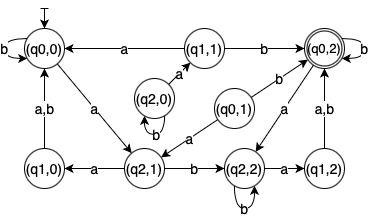
\includegraphics[scale=0.75]{NEA-Konstruktion}  
	


\newpage